

\subsubsection{MQTT broker}
MQTT( MQ telemetru transport) es un protocolo de mensajería comúnmentete
utilizado en sistema o dispositivos IoT, basado en el patron
publish/subscribe, donde los mensajes son publicados en un tópico de un MQTT
broker que se encarga de distribuirlos a todos sus subscriptores que se hayan
subscrito al tópico . 
\begin{figure}[H]
    \centering
    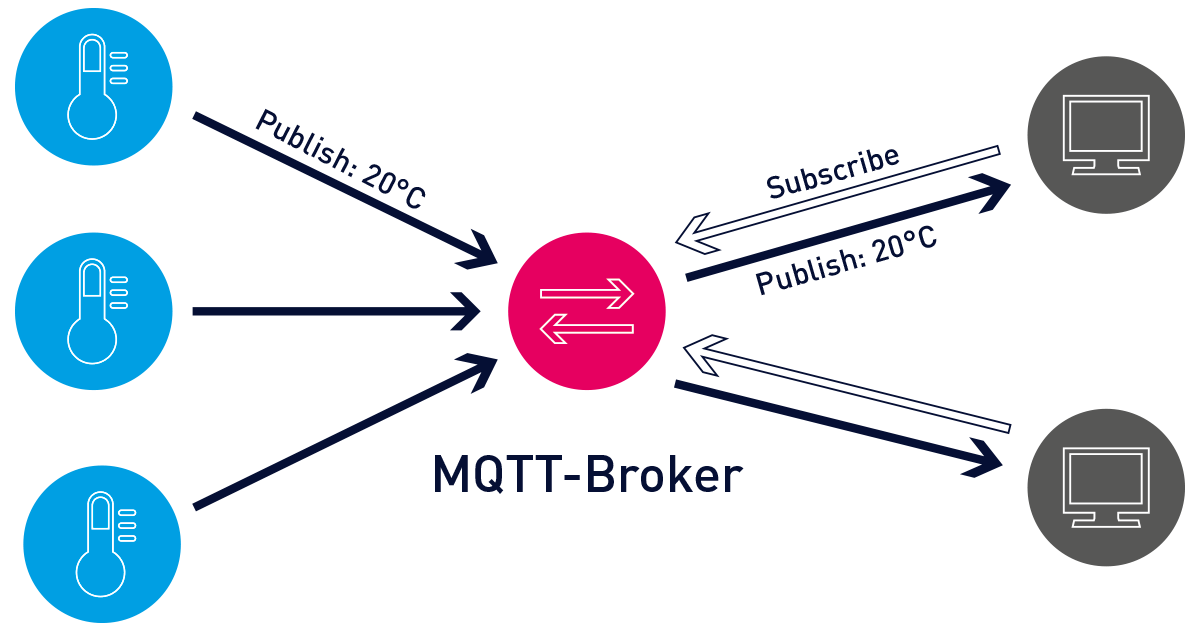
\includegraphics[width=\textwidth, keepaspectratio,
    height=7cm]{images/mqtt-architecture.png}
    \caption{Arquitectura de un broker MQTT}
    \label{fig:mqtt_arquitecture}
\end{figure}

Para la estación de monitoreo se esta haciendo uso de un borker  MQTT de codigo
abiero llamado \href{http://mosquitto.org}{eclipse mosquito}.

\subsubsection{Telegraf}
Telegraf es un agente que nos permite recopilar y reportar métricas. Las
métricas recogidas se pueden enviar a almacenes de datos, colas de mensajes o
servicios como: InfluxDB, Graphite, OpenTSDB, Datadog, Kafka, MQTT, NSQ, entre
otros.

\begin{figure}[H]
    \centering
    
\includegraphics[width=\textwidth, keepaspectratio,
    height=5cm]{images/logo-telegraf-1.jpg}
    \caption{telegraf}
    \label{fig:logo_telegraf}
\end{figure}

\subsubsection{InfluxDB}
Es un sistema gestor de bases de datos diseñado para almacenar bases
de datos de series temporales (TSBD - Time Series Databases). Estas bases de
datos se suelen utilizar en aplicaciones de monitorización, donde es necesario
almacenar y analizar grandes cantidades de datos con marcas de tiempo, como
pueden ser datos de uso de cpu, uso memoria, datos de sensores de IoT, etc.

\begin{figure}[H]
    \centering
    
\includegraphics[width=\textwidth, keepaspectratio,
    height=5cm]{images/Influxdb_logo.svg_.png}
    \caption{Influxdb}
    \label{fig:logo_influx}
\end{figure}
\subsubsection{Grafana}
Es un servicio web que que permite visualizar en un panel de control
los datos almacenados en InfluxDB y otros sistemas gestores de bases de datos
de series temporales.
\begin{figure}[H]
    \centering
    
\includegraphics[width=\textwidth, keepaspectratio,
    height=5cm]{images/1200px-Grafana_logo.svg.png}
    \caption{Grafana}
    \label{fig:grafana}
\end{figure}



